%Chapter 1 
\chapter{Let's get it started} 
\label{Chap:setup}
\ifpdf
    \graphicspath{{Chapters/OneCh/Figs/Raster/}{Chapters/OneCh/Figs/PDF/}{Chapters/OneCh/Figs/}}
\else
    \graphicspath{{Chapters/OneCh/Figs/Vector/}{Chapters/OneCh/Figs/}}
\fi
Now I'm empty and you've to work a lot, but at the end it will be like Fig.~\ref{Fig:PHD}. Place all the figures in \textbf{Chapters/OneCh/Figs}. Chapter1 is an example for the structure, you can use it as a template for other chapters. 

\begin{figure}
\begin{center}
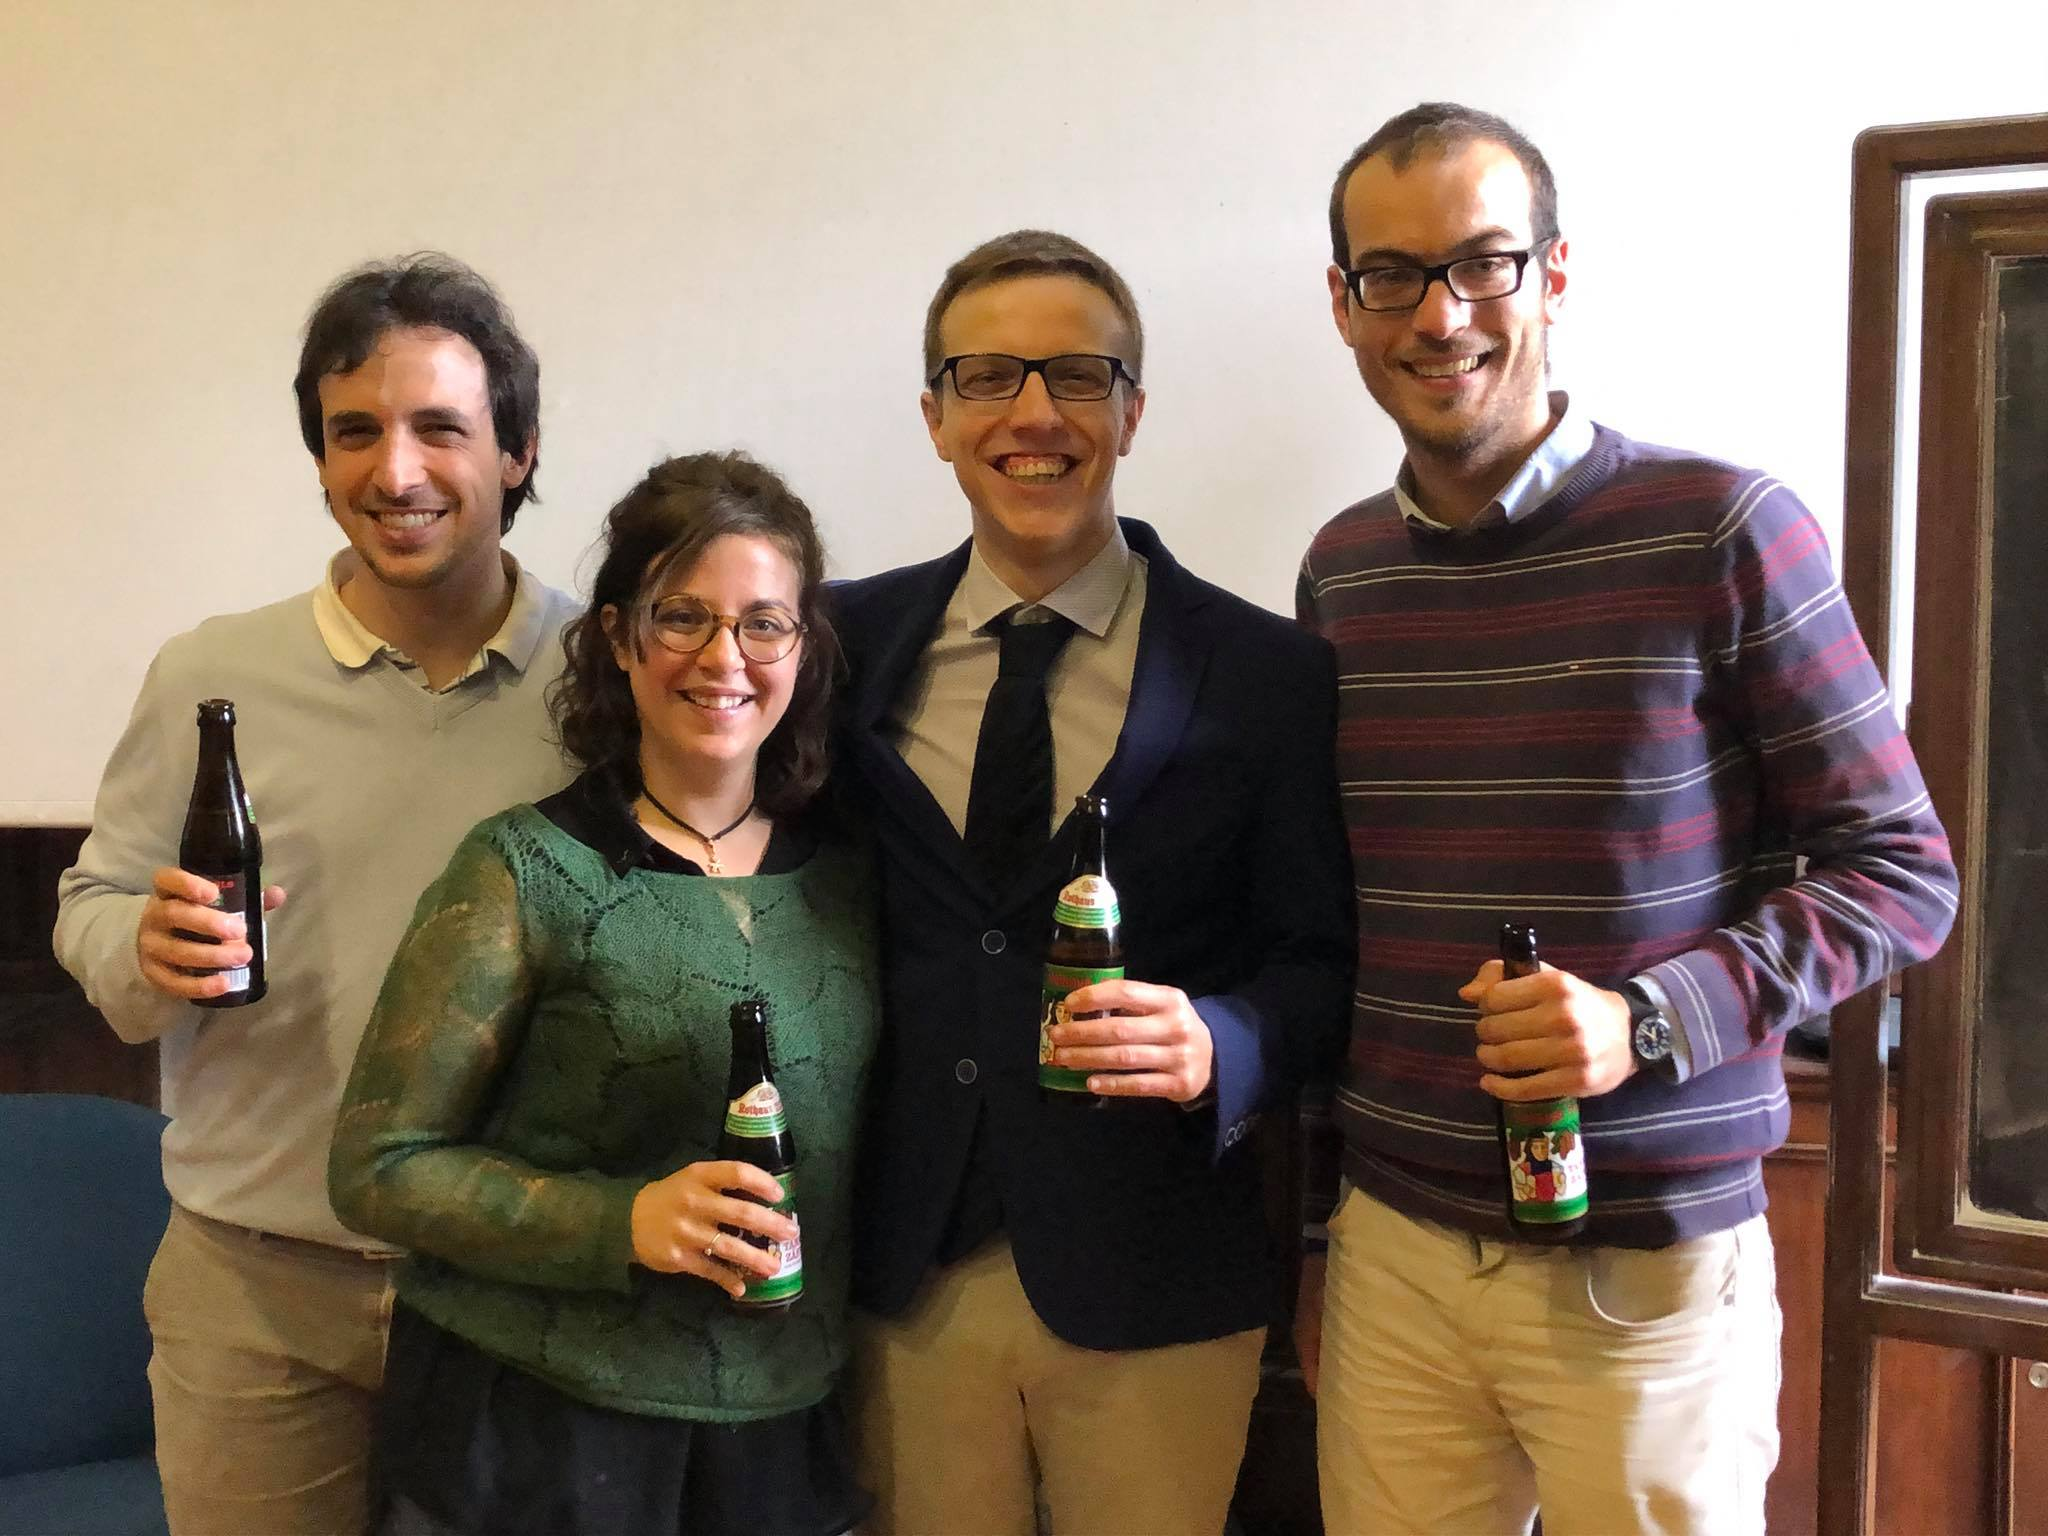
\includegraphics[width=14.8cm]{End}
\caption{Torino, A.D. 2018. Young PhDs celebrating the OktoberFest}
\label{Fig:PHD}
\end{center}
\end{figure}
\section{Tips of the day} 
If you have variables or functions or in general equation-like text that repeats often in your text (e.g. asymmetries, TMDs, etc..) I would strongly advise to define them in the main file thesis.txt declaring an alias for them. In this way you can recall them easily while writing, w/o needing of rewriting the full formula every time (and avoiding in this way a lot of typos that then drives the reader mad! :) ) \\ 
Remember that to recompile you have always to use the main file thesis.txt. Compiling single chapters will give you errors. 
If you want to speed up the compilation, you can temporarily comment out some chapter (but you will maybe get errors for missing references). 

\subsection{Sub-example}

For example , $f_{1,T}^{\, q\perp}(x,\mathbf{k_T})$ here is simply defined as \siv  !  
This allows you to save a lot of time and to keep your notation uniform along the thesis (your referees and supervisors will love you!)

\section{Bibliography} 
Remember that, when you add something to the bibliography, you have first to recompile it and then recompile twice the thesis to have your new references appearing in the correct way. Basically:
\begin{itemize}
\item BibTex thesis.txt
\item PDFLaTex thesis.txt
\item PDFLaTex thesis.txt
\end{itemize} 
The bibliography file sits in \textbf{References/references.bib}

Let's cite an article of Matthias!  \cite{Perdekamp:2015vwa}

\section{Conclusions} 
Remember the basic rule to work with latex. Your problem has been met by already $n$ users. So, just google it! 
Good luck! And if you need some help, don't hesitate to ask me. 

Riccardo 
